\section{Introduction}\label{sec:intro}
Introduction starts here.

\subsection{Table}
\begin{table}[tbh]
  \centering
  \caption{Table Example}\label{tbl:ex}
  \begin{tabular}{|ccc|}
    \hline
	Column 1 & Column 2 & Column 3	\\ \hline\hline
	Column 1 & Column 2 & Column 3	\\ \hline
    Column 1 & Column 2 & Column 3	\\ \hline
  \end{tabular}
\end{table}

\subsection{Figure}
\begin{figure}[!tbh]
	\centering
	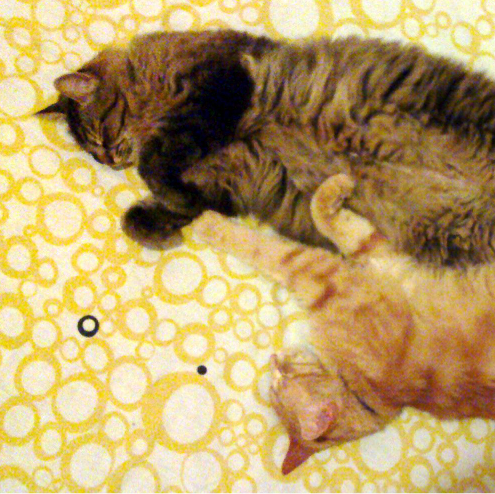
\includegraphics[scale=0.5]{./figures/cats.png}
\caption{Figure Example}
\label{fig:ex}
\end{figure}

\subsection{Code}
\begin{lstlisting}[caption=Code Example \label{lst:code_ex}]
int foo(int a, int b) {
  int sum = 0;
  for (int i = 0; i < a; i++)
    for (int j = 0; j < b; j++)
      sum++;
  return sum;
}
\end{lstlisting}

\subsection{Theorem and Equation}

\begin{theorem}
This is the first theorem
\end{theorem}
\begin{proof}
The proof.
\end{proof}

\begin{theorem}
This is the second theorem
\end{theorem}

\subsection{Reference}
\cite{ref1,ref2,ref3,ref4,ref5,ref6}
